\documentclass[a4paper,10pt]{article}
\usepackage{fontspec}
\usepackage{setspace}
\usepackage{booktabs}
\usepackage{amsmath}
\usepackage{cancel}
\usepackage{graphicx}
\usepackage{biblatex}
\usepackage{float}

\setmainfont{arial}
\setstretch{1.15}
\addbibresource{references.bib}

\title{Image Preprocessing}
\author{Arif Suganda\\
        Tadulako University\\
        \texttt{f5522530002@untad.ac.id}
}

\begin{document}
\maketitle

\section{Image Quality}

In this digital age image is one of the highest data collected in the world, 
from digital camera to analog camera the process of taking an image plagued by many problem, 
wether it is image noise or image quality degradation there are exist solutions that can be perform to restore and even enhance the quality of an image.
This experiment will explore some of options avalable for restoration and enhancement of bad quality image.

For this experiment we will be using an image often used to performed digital image processing, the image can be seen in Figure~\ref*{fig:image}

\begin{figure}[H]
    \centering
    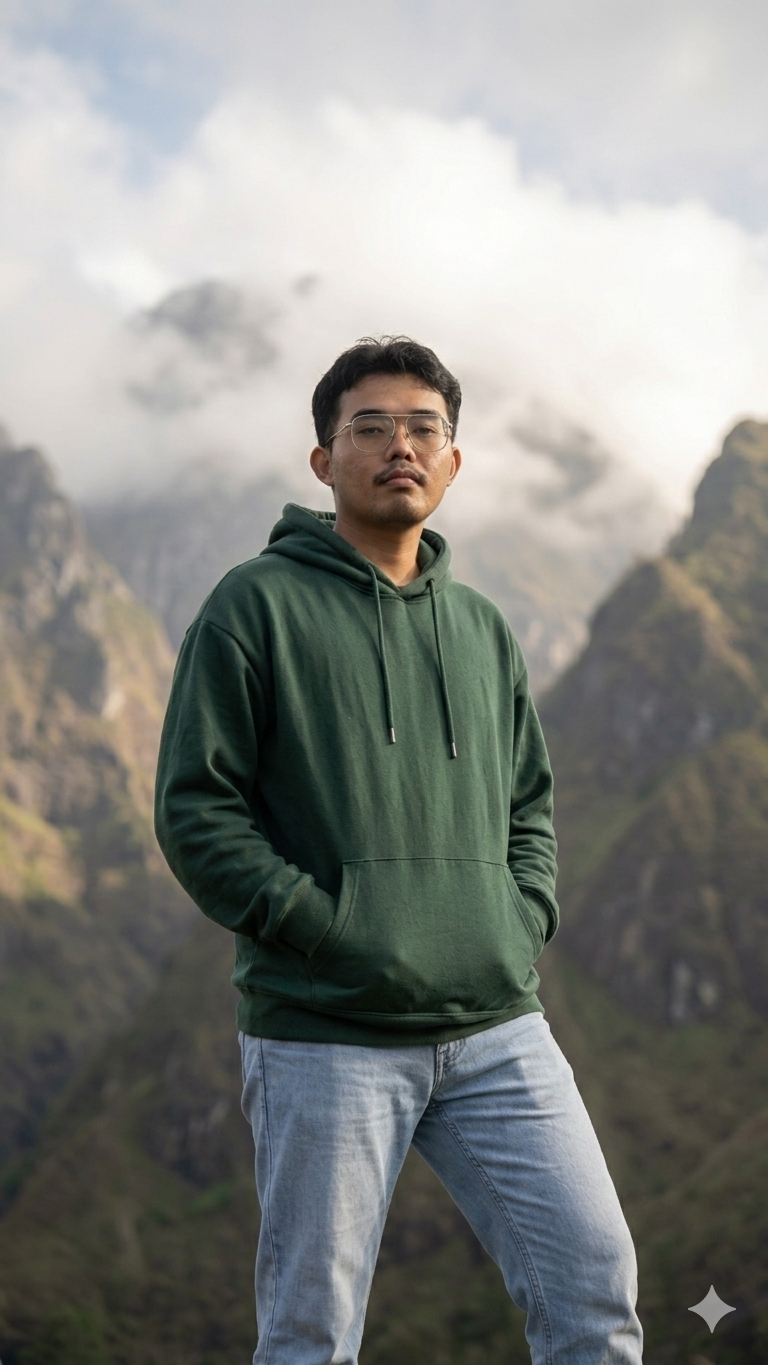
\includegraphics[width=0.4\textwidth]{image.png} 
    \caption{Gemini generated image}\label{fig:image}
\end{figure}

\section{Image degradation}

Image degradation is a problem that occurs in a digital image that damage image quality. Examples of image degradation can be seen in example below.
\subsection{Salt and Pepper Noise}
Salt and pepper noise is represented by maximum or minimum value of a pixel such as white for salt and black for pepper.
Salt and pepper noise can be added using this command:
\begin{verbatim}
from skimage.util import random_noise
import skimage.io as io
import matplotlib.pyplot as plt

image_path = 'image.png'
image = io.imread(image_path)

sp_img = random_noise(image, mode='s&p', amount=0.05)
plt.figure(figsize=(8, 8))
plt.imshow(sp_img)
plt.axis('off')
plt.show()
\end{verbatim}

The result can be seen in Figure~\ref*{fig:salt_and_pepper}

\begin{figure}[H]
    \centering
    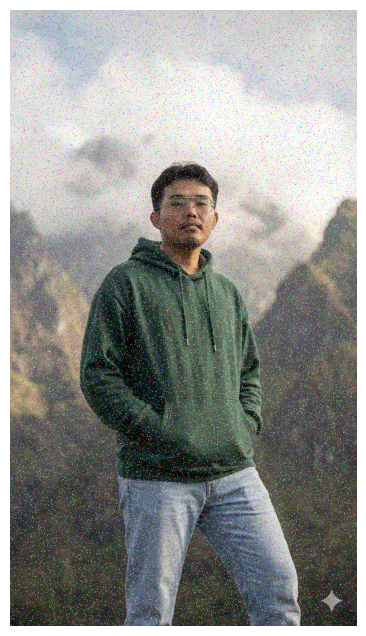
\includegraphics[width=0.4\textwidth]{salt_and_pepper.png} 
    \caption{Salt and pepper noise}\label{fig:salt_and_pepper}
\end{figure}

\subsection{Poisson noise}
Poisson noise is a noise that occurs due to fluctuation of light when an image is taken.
Poisson noise can be added using this command:
\begin{verbatim}
poisson = random_noise(image, mode='poisson')
plt.figure(figsize=(8, 8))
plt.imshow(poisson)
plt.axis('off')
plt.show()
\end{verbatim}

The result can be seen in Figure~\ref*{fig:poisson}

\begin{figure}[H]
    \centering
    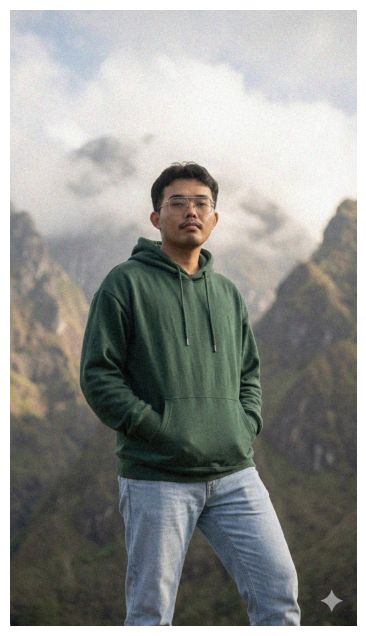
\includegraphics[width=0.4\textwidth]{poisson.png} 
    \caption{Poisson noise}\label{fig:poisson}
\end{figure}

\section{Noise Reduction}
Noise reduction is a restoration technique used on a damage image, adding or changing each pixel with a new value.

\subsection{Median filter}
Median filter is used to change each pixel value with the median value of its neighboring pixel.
This process will restore a damage in individual pixel without losing the overall image edge sharpness.
Implementation can be seen using this command:
\begin{verbatim}
sp_img_32 = sp_img.astype(np.float32)
sp_denoise = cv2.medianBlur(sp_img_32, 5)

poisson_img_32 = poisson.astype(np.float32)
poisson_denoise = cv2.medianBlur(poisson_img_32, 5)

fig, axes = plt.subplots(nrows=2, ncols=2, figsize=(8, 8))
axes[0][0].imshow(sp_img_32)
axes[0][0].set_title('Salt and Pepper noise')
axes[0][1].imshow(sp_denoise)
axes[0][1].set_title('Median filter')
axes[1][0].imshow(poisson_img_32)
axes[1][0].set_title('Poisson noise')
axes[1][1].imshow(poisson_denoise)
axes[1][1].set_title('Median filter')
for row in axes:
    for ax in row:
        ax.axis('off')
plt.tight_layout()
plt.show()
\end{verbatim}

\noindent
With result can seen in Figure~\ref*{fig:median_filter}

\begin{figure}[H]
    \centering
    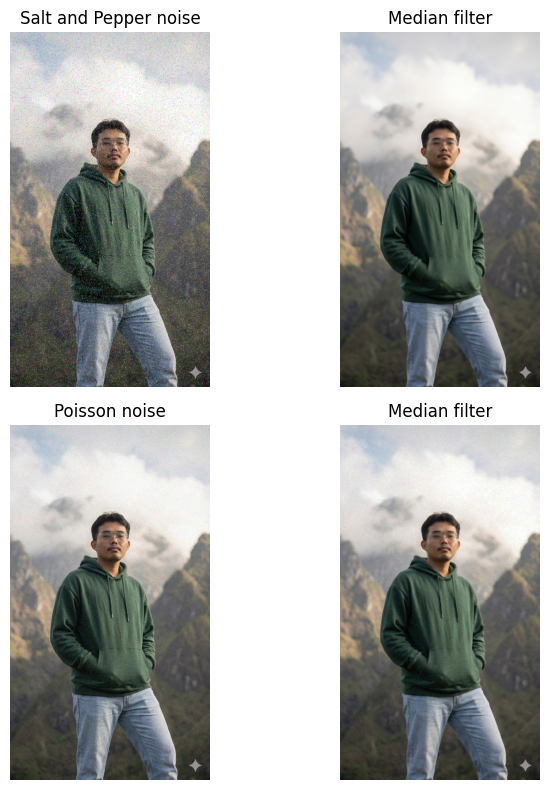
\includegraphics[width=1\textwidth]{median_filter.png} 
    \caption{Median filter comparison}\label{fig:median_filter}
\end{figure}

\subsection{Mean filter}
Mean filter is used to change each pixel value with the average value of its neighboring pixel resulting in general smoothing of the image.
Implementation can be seen using this command:
\begin{verbatim}
sp_img_32 = sp_img.astype(np.float32)
sp_denoise = cv2.blur(sp_img_32, (3, 3))

poisson_img_32 = poisson.astype(np.float32)
poisson_denoise = cv2.blur(poisson_img_32,(3, 3))

fig, axes = plt.subplots(nrows=2, ncols=2, figsize=(8, 8))
axes[0][0].imshow(sp_img_32)
axes[0][0].set_title('Salt and Pepper noise')
axes[0][1].imshow(sp_denoise)
axes[0][1].set_title('Mean filter')
axes[1][0].imshow(poisson_img_32)
axes[1][0].set_title('Poisson noise')
axes[1][1].imshow(poisson_denoise)
axes[1][1].set_title('Mean filter')
for row in axes:
    for ax in row:
        ax.axis('off')
plt.tight_layout()
plt.show()
\end{verbatim}

\noindent
With result can seen in Figure~\ref*{fig:mean_filter}

\begin{figure}[H]
    \centering
    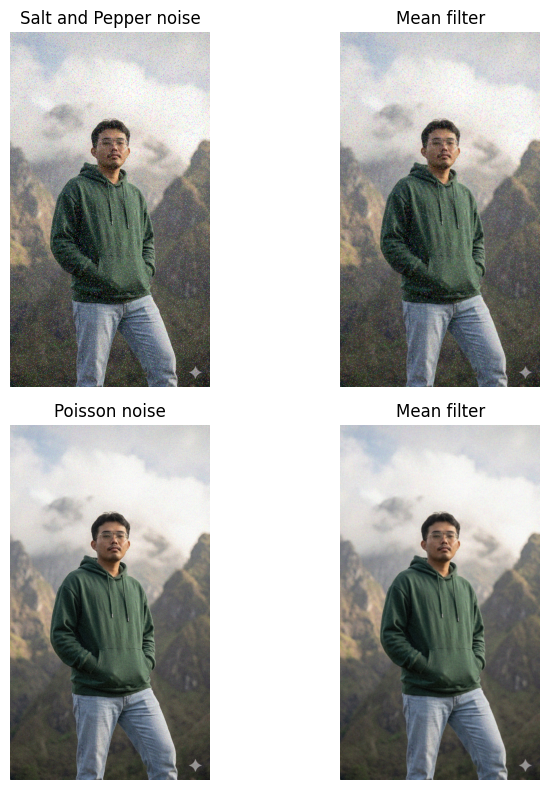
\includegraphics[width=1\textwidth]{mean_filter.png} 
    \caption{Mean filter comparison}\label{fig:mean_filter}
\end{figure}

\subsection{Gaussian filter}
Gaussian filter change each pixel with a weighted average of its neighbors, the closer pixels get higher weights based on a bell-curve (Gaussian) distribution, resulted in more natural smooting.
Implementation can be seen using this command:
\begin{verbatim}
sp_img_32 = sp_img.astype(np.float32)
sp_denoise = cv2.GaussianBlur(sp_img_32, (3, 3), 0)

poisson_img_32 = poisson.astype(np.float32)
poisson_denoise = cv2.GaussianBlur(poisson_img_32, (3, 3), 0)

fig, axes = plt.subplots(nrows=2, ncols=2, figsize=(8, 8))
axes[0][0].imshow(sp_img_32)
axes[0][0].set_title('Salt and Pepper noise')
axes[0][1].imshow(sp_denoise)
axes[0][1].set_title('Gaussian filter')
axes[1][0].imshow(poisson_img_32)
axes[1][0].set_title('Poisson noise')
axes[1][1].imshow(poisson_denoise)
axes[1][1].set_title('Gaussian filter')
for row in axes:
    for ax in row:
        ax.axis('off')
plt.tight_layout()
plt.show()
\end{verbatim}

\noindent
With result can seen in Figure~\ref*{fig:gaussian_filter}

\begin{figure}[H]
    \centering
    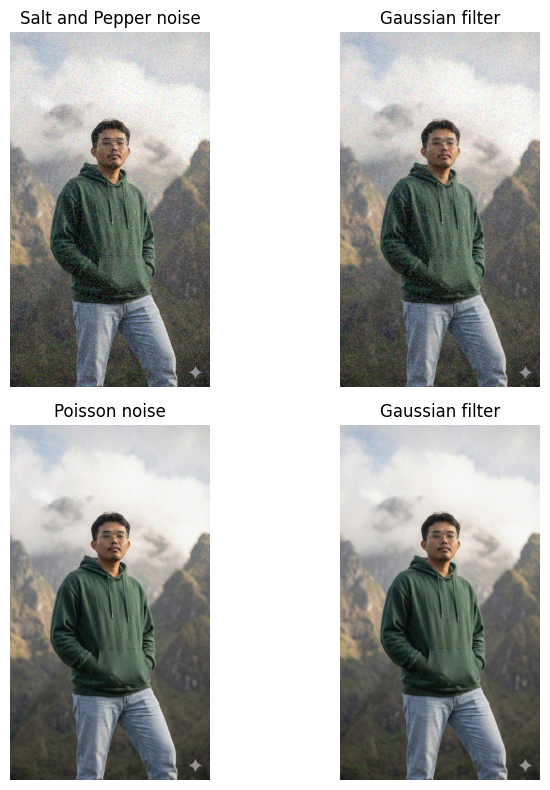
\includegraphics[width=1\textwidth]{gaussian_filter.png} 
    \caption{Gaussian filter comparison}\label{fig:gaussian_filter}
\end{figure}

\section{Image Enhancement}
Image enhancement works by changing the overall pixel value to better suited for processing.
From model training to printing image enhancement increase the visibility of an image or enhance the certain feature within the image.

\subsection{Normalization}
Normalization works by limiting the values of the pixels into minimum and maximum value.

\subsection{Resizing}
Resizing works by estimating new pixel values from existing image when changing image dimension. 
There are two ways of resizing, make it larger (upscaling) and make it smaller (downscaling).
This implementation will be using resizing and nomalization, which using this command:
\begin{verbatim}
img = image.astype(np.float32)

downscale = cv2.resize(img, (0, 0), fx=0.5, fy=0.5)
upscale = cv2.resize(img, (0, 0), fx=1.5, fy=1.5)
img_normalized = img / 255.0
upscale_normalized = upscale / 255.0
downscale_normalized = downscale / 255.0

fig, axes = plt.subplots(ncols=3, figsize=(8, 8))
axes[0].imshow(img_normalized)
axes[0].set_title('Original')
axes[1].imshow(upscale_normalized)
axes[1].set_title('Upscale')
axes[2].imshow(downscale_normalized)
axes[2].set_title('Downscale')
plt.tight_layout()
plt.show()
\end{verbatim}
\noindent
With result can be show in Figure~\ref*{fig:resizing}, looking at the y axis we can see the number of pixel increase and decrease.
\begin{figure}[H]
    \centering
    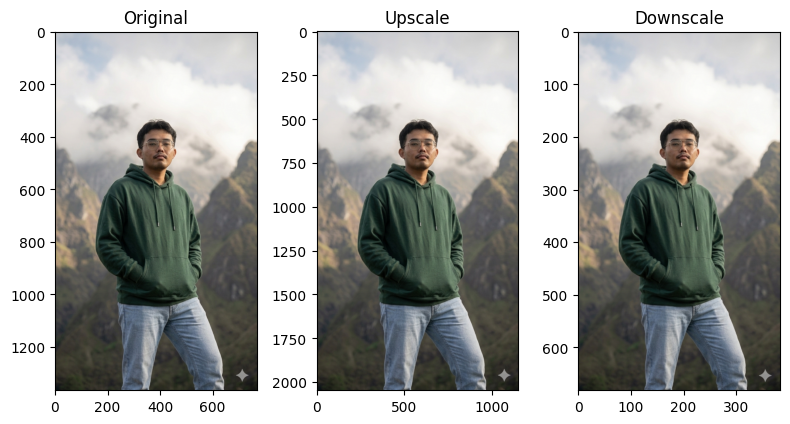
\includegraphics[width=1\textwidth]{resizing.png} 
    \caption{Resizing}\label{fig:resizing}
\end{figure}

\subsection{Color conversion}
Color conversion works by changing the color of an image into another color channel, such as grayscale, HSV or YUV.
The following example is to change the color conversion from RGB to grayscale.
\begin{verbatim}
img_bgr = cv2.imread(image_path)
gray_img = cv2.cvtColor(img_bgr, cv2.COLOR_BGR2GRAY)

fig, axes = plt.subplots(ncols=2, figsize=(8, 8))
axes[0].imshow(image)
axes[0].set_title('Original')
axes[1].imshow(gray_img, cmap='gray')
axes[1].set_title('Grayscale')
plt.tight_layout()
plt.show()
\end{verbatim}

\noindent
With result shown in Figure~\ref*{fig:grayscale}.
\begin{figure}[H]
    \centering
    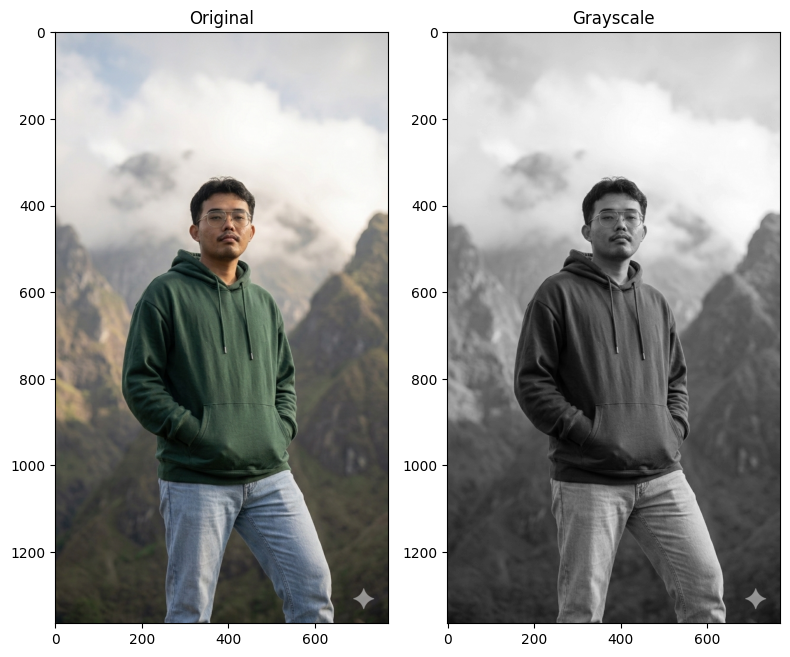
\includegraphics[width=0.6\textwidth]{grayscale.png} 
    \caption{Grayscale}\label{fig:grayscale}
\end{figure}

\subsection{Histogram equalization}
Histogram equalization works by stretching each pixel color value into acceptable range between 0 to 255 to improve contrast of an image.
An image using RGB image consist of 3 pixel color values, which mean that color distribution must be observed using 3 color channel.
The following command used to observe color distribution of RGB image:
\begin{verbatim}
import cv2
import matplotlib.pyplot as plt

img = cv2.imread(image_path)
img_rgb = cv2.cvtColor(img, cv2.COLOR_BGR2RGB)

# Plot histogram for each channel
colors = ('r', 'g', 'b')
plt.figure(figsize=(10, 4))

for i, color in enumerate(colors):
    hist = cv2.calcHist([img], [i], None, [256], [0, 256])
    plt.plot(hist, 
    color=color, label=f'{color.upper()} channel')

plt.title('RGB Color Histogram')
plt.xlabel('Pixel Value (0-255)')
plt.ylabel('Frequency')
plt.legend()
plt.tight_layout()
plt.show()
\end{verbatim}

\noindent
Distribution can be seen in Figure~\ref*{fig:rgb_color_histogram}
\begin{figure}[H]
    \centering
    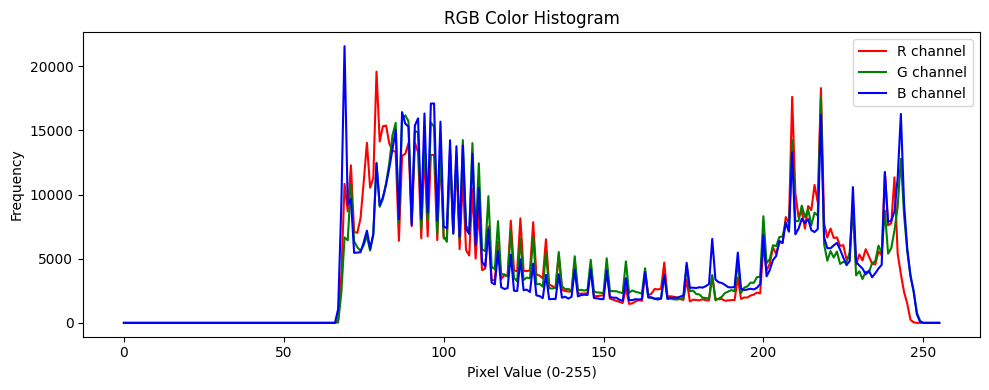
\includegraphics[width=1\textwidth]{rgb_color_histogram.png} 
    \caption{RGB color histogram}\label{fig:rgb_color_histogram}
\end{figure}

As we can see above the distribution of rgb color consentrated mostly in middle of the range.
Using the command below to equalize the color of each RGB channel:
\begin{verbatim}
r, g, b = cv2.split(img_rgb)
r_eq = cv2.equalizeHist(r)
g_eq = cv2.equalizeHist(g)
b_eq = cv2.equalizeHist(b)

img_eq = cv2.merge([r_eq, g_eq, b_eq])
fig, axes = plt.subplots(ncols=2, figsize=(8, 8))
axes[0].imshow(image)
axes[0].set_title('Original')
axes[1].imshow(img_eq)
axes[1].set_title('Histogram equalization')
plt.tight_layout()
plt.show()
\end{verbatim}

\noindent
Resulted in distribution of colors in the image, which can be seen in Figure~\ref*{fig:rgb_color_histogram1}, with result shown in Figure~\ref*{fig:histogram_equalization}.
\begin{figure}[H]
    \centering
    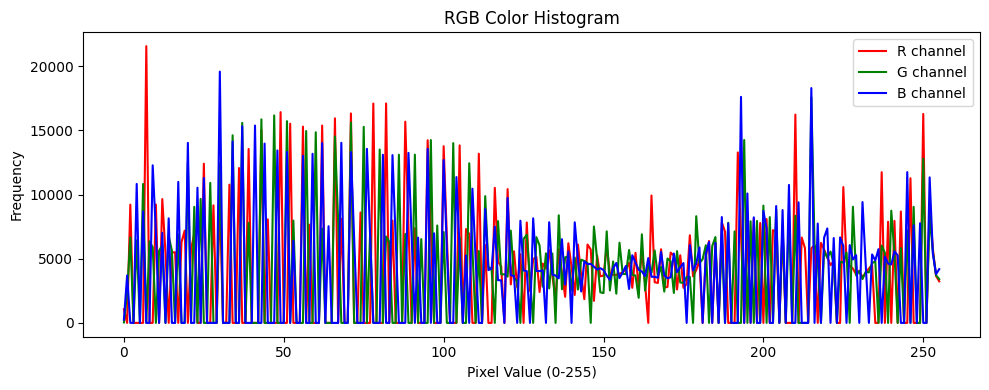
\includegraphics[width=1\textwidth]{rgb_color_histogram1.png} 
    \caption{Distributed RGB color histogram}\label{fig:rgb_color_histogram1}
\end{figure}
\begin{figure}[H]
    \centering
    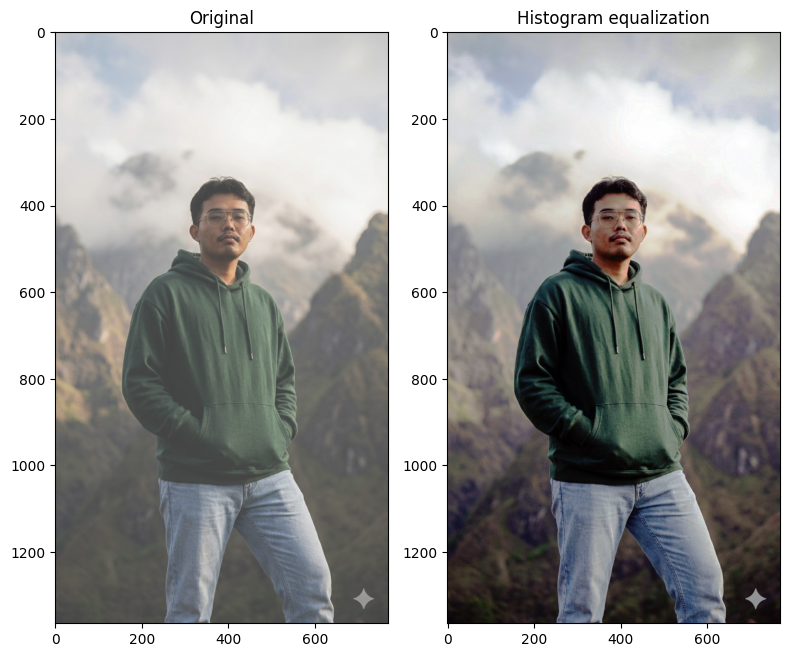
\includegraphics[width=1\textwidth]{histogram_equalization.png} 
    \caption{Histogram equalization}\label{fig:histogram_equalization}
\end{figure}

\section{Discussion}
Shown in Figure~\ref*{fig:comparison} about comparison between multiple filter, each filter resulted in slightly different result.
In salt and pepper noise median filter get a better result than other filter,
the reason is because noise rarely contribute to the changing of a pixel.
The salt and pepper noise value is highest and the lowest value which is white and black, 
when sorted their order is often at the first or the last pixel value and rarely chosen.

Poison noise difference is that the noise contribute to all pixel, the result of mean and median filter will be influenced by the noise.
However the gaussian filter works better because it has a curved distribution which gives the variation of each pixel, rather than overall pixel.

\begin{figure}[H]
    \centering
    
\includegraphics[width=1\textwidth]{comparison.png} 
    \caption{Filter comparison}\label{fig:comparison}
\end{figure}


\end{document}